\clearpage

\vspace{20mm}

\begin{minipage}{16cm}
%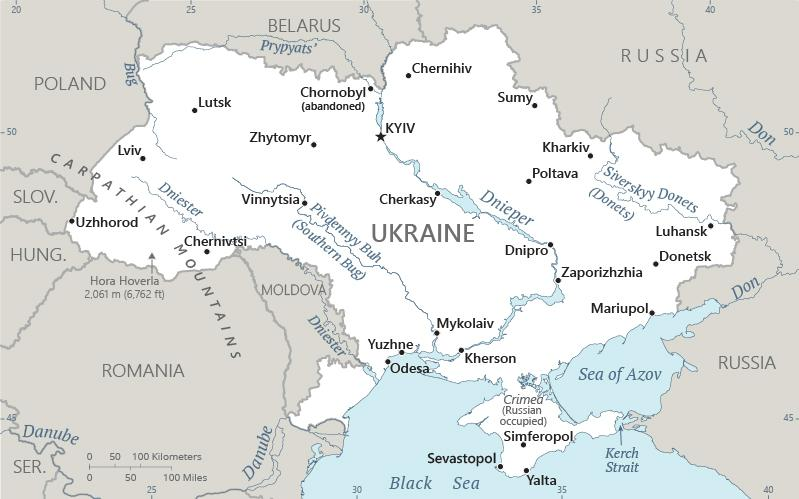
\includegraphics[width=0.8\paperwidth]{Pictures/other/ukraine-map.jpg}
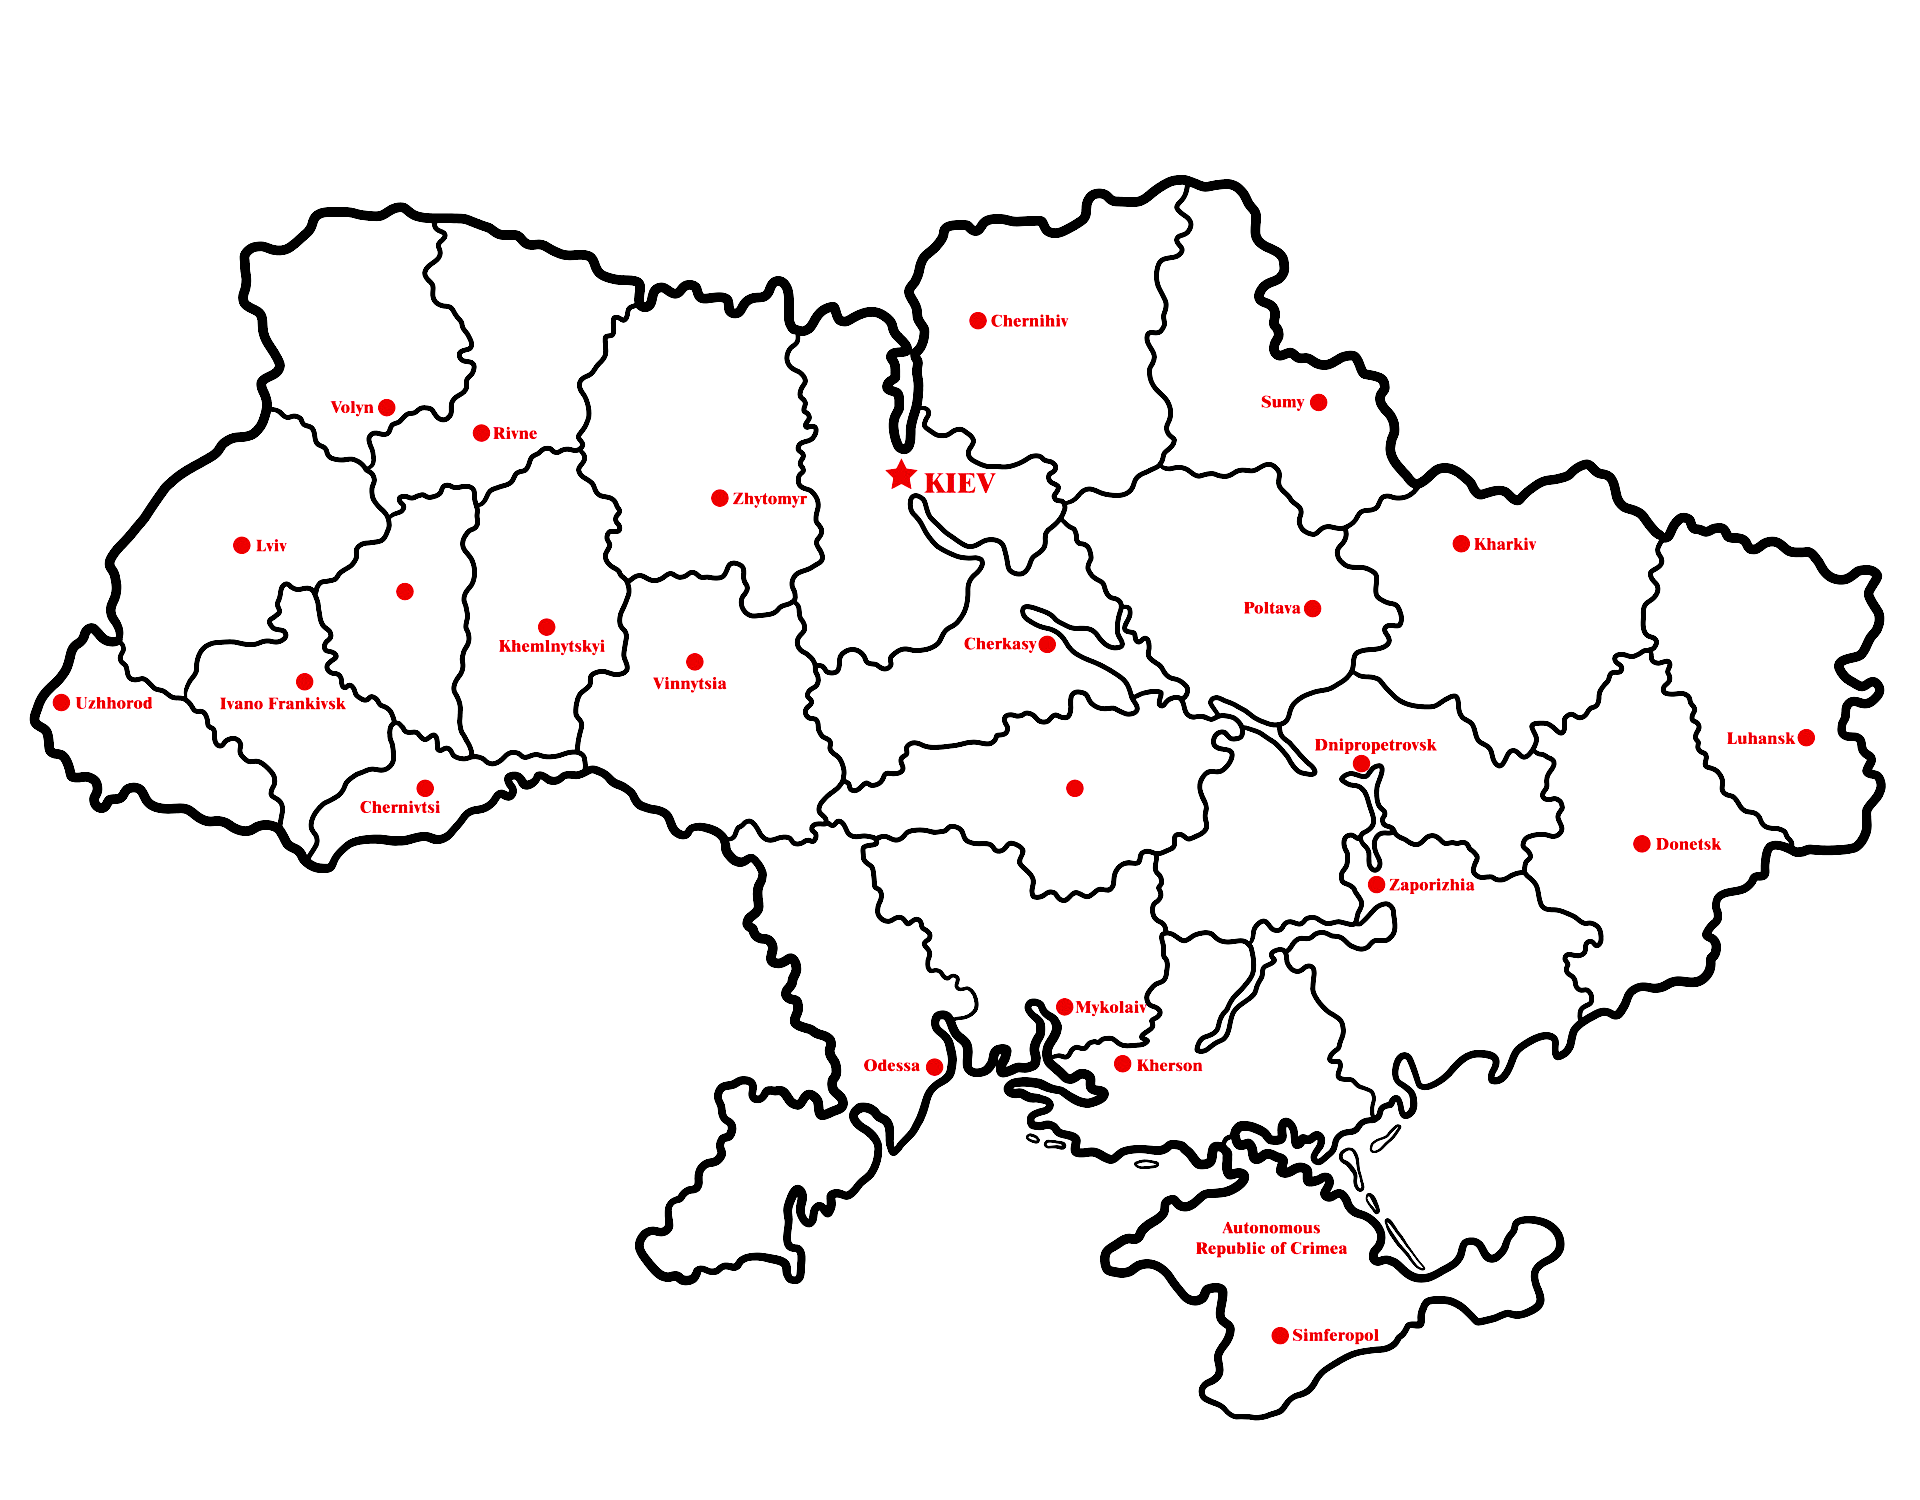
\includegraphics[width=0.8\paperwidth]{Pictures/other/ukrainian-map-bw.png}
\end{minipage}

\clearpage

\part{About Ukraine}

\chapter{Ukrainian Culture}

\clearpage

\section{Independence Day of Ukraine}

\textit{From Wikipedia}\footnote{\url{https://en.wikipedia.org/wiki/Independence_Day_of_Ukraine}}

The \textbf{Independence Day of Ukraine} (Ukrainian: 
\begin{ukrainian}День Незалежності України\end{ukrainian},
romanized: Den' Nezale\~znosti Ukrajiny) is a state holiday, celebrated on \textbf{24 August}
in commemoration of the Declaration of Independence from the Soviet Union.

The current form of the holiday was first celebrated on 16 July 1991, as the first
anniversary of the Declaration of State Sovereignty of Ukraine passed by the
Verkhovna Rada (Ukraine's parliament) in 1990.
The Declaration of Independence was issued on 24 August 1991, 
and confirmed by the referendum of 1 December 1991.

\section{The Ukrainian Flag}

\textit{From Wikipedia}\footnote{\url{https://en.wikipedia.org/wiki/Flag_of_Ukraine}}

The \textbf{National Flag of Ukraine} consists of equally sized horizontal bands of blue and yellow.

The blue and yellow bicolor flag was first seen during the 1848 Spring of Nations in Lemberg (Lviv),
the capital of the Kingdom of Galicia and Lodomeria within the Austrian Empire. 
It was later adopted as a state flag by the short-lived Ukrainian People's Republic,
the West Ukrainian People's Republic, and the Ukrainian State following the Russian Revolution.

In March 1939, it was also adopted by Carpatho-Ukraine. However, when Ukraine was part of the Soviet
Union, the use of the bicolor flag was banned.  When the Soviet Union dissolved in 1991, 
the bicolor flag gradually returned to use before being officially adopted again on 
28 January 1992 by the Ukrainian parliament.

Ukraine celebrates the \textbf{Day of the National Flag} on \textbf{23 August}.

\photo{Pictures/other/ukraine-flag.jpg}

\newpage

\section{State Anthem of Ukraine}

\begin{center}
\begin{ukrainian}
\begin{tabular}{l}
Ще не вмерла України і слава, і воля, \\
Ще нам, браття молодії, усміхнеться доля. \\
Згинуть наші воріженьки, як роса на сонці. \\
Запануєм і ми, браття, у своїй сторонці. \\
\\
Душу й тіло ми положим за нашу свободу, \\
І покажем, що ми, браття, козацького роду. \\
\end{tabular}
\end{ukrainian}
\end{center}

\vspace{5mm}
The words of the State Anthem of Ukraine are a slightly modified version of the
first verse and chorus of the patriotic song "Shche ne vmerla Ukraina", 
written by Pavlo Chubynskyi, a prominent ethnographer from Kyiv.
The words can be traced back to one of the parties of Pavlo Chubynskyi
that occurred during the autumn of 1862.

In 1863, Mykhailo Verbytskyi, a Ukrainian composer and Greek Catholic priest, 
composed music to accompany Chubynskyi's lyrics.

A competition was held for a national anthem following Ukraine's secession from the Soviet Union.
"Shche ne vmerla Ukraina" was officially adopted by Ukraine's Verkhovna Rada (parliament) on 
15 January 1992. The official lyrics were adopted on 6 March 2003 by the
Law on the State anthem of Ukraine.

\textbf{In English}

\begin{center}
\begin{tabular}{l}
The glory and freedom of Ukraine has not yet perished\\
Luck will still smile on us brother-Ukrainians.\\
Our enemies will die, as the dew does in the sunshine,\\
and we, too, brothers, we'll live happily in our land.\\
\\
We'll not spare either our souls or bodies to get freedom\\
and we'll prove that we brothers are of Kozak kin.\\
\end{tabular}
\end{center}

\clearpage 

\newpage


